\begin{frame}
\begin{center}
\vspace{-2em}
\only<1>{%
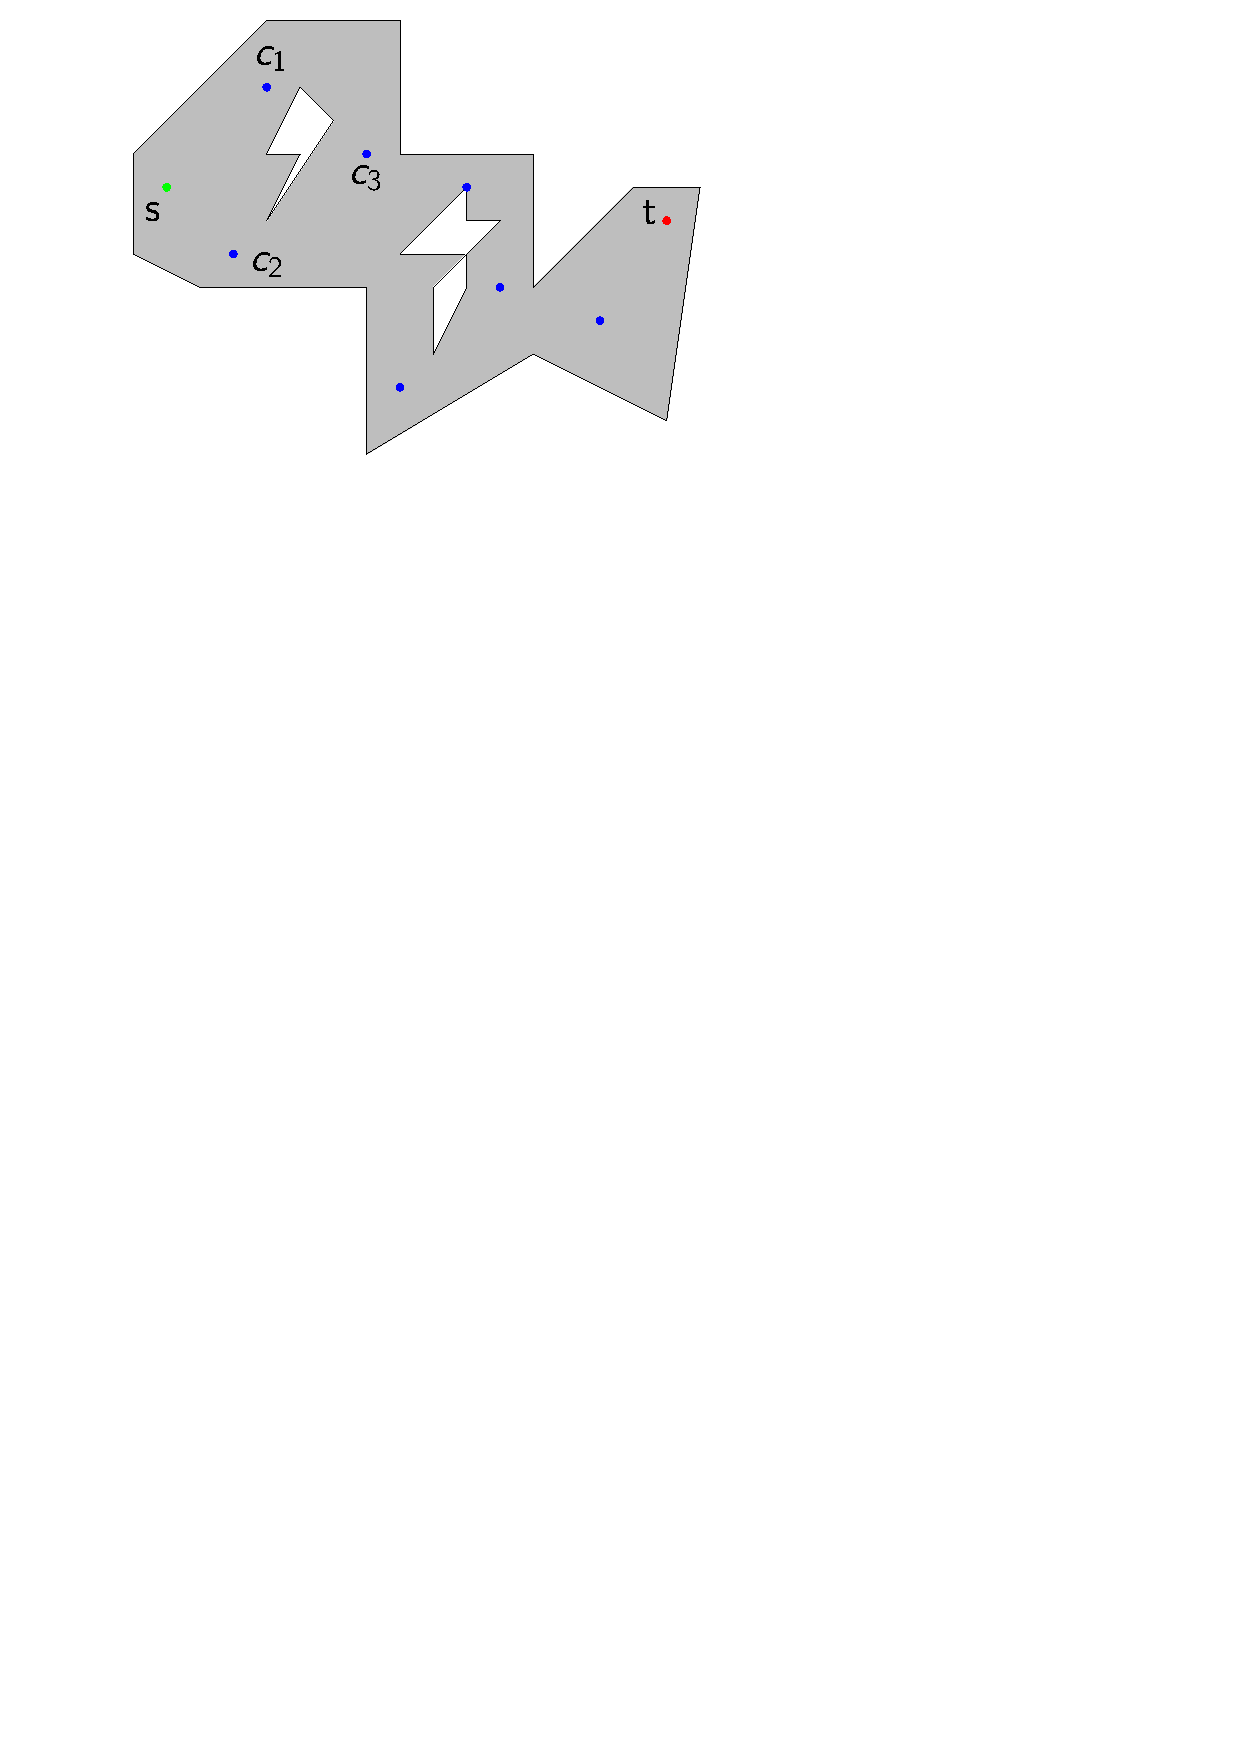
\includegraphics[page=1,height=150pt]{graphics/input1.pdf}%
}%
\only<2>{%
\includegraphics[page=2,height=150pt]{graphics/input1.pdf}%
}%
\end{center}

\begin{itemize}
\item Electric robot is in a warehouse polygon $P$, starting at green location $s$
\item Range of $r$, recharge at blue charging stations $c \in C$
\item What is the shortest path to red exit location $t$
\end{itemize}

\end{frame}

\begin{frame}{Overview}
Computing visibility graphs
\\[2em]
Computing shortest route
\\[2em]
Possible optimizations
\end{frame}

\begin{frame}{Visibility Graph}

\vspace{-1em}
\begin{mydef}{}
Given a set of points $S$ inside $P$, the \textbf{visibility graph}
of $S$ is the undirected graph $G_S = (S, E)$ with edges
$E = \{\{a, b\}\ | \  \overline{ab} \subseteq P \}$
\end{mydef}

%\begin{itemize}
%\item Let $V$ be the vertices of the polygon $P$
%\item
We are interested in the point set $S = P \cup C \cup \{s, t\}$
%\item If we know the visibility graph $G_M$, our problem reduces to the
%corresponding graph problem
%\end{itemize}
\begin{center}
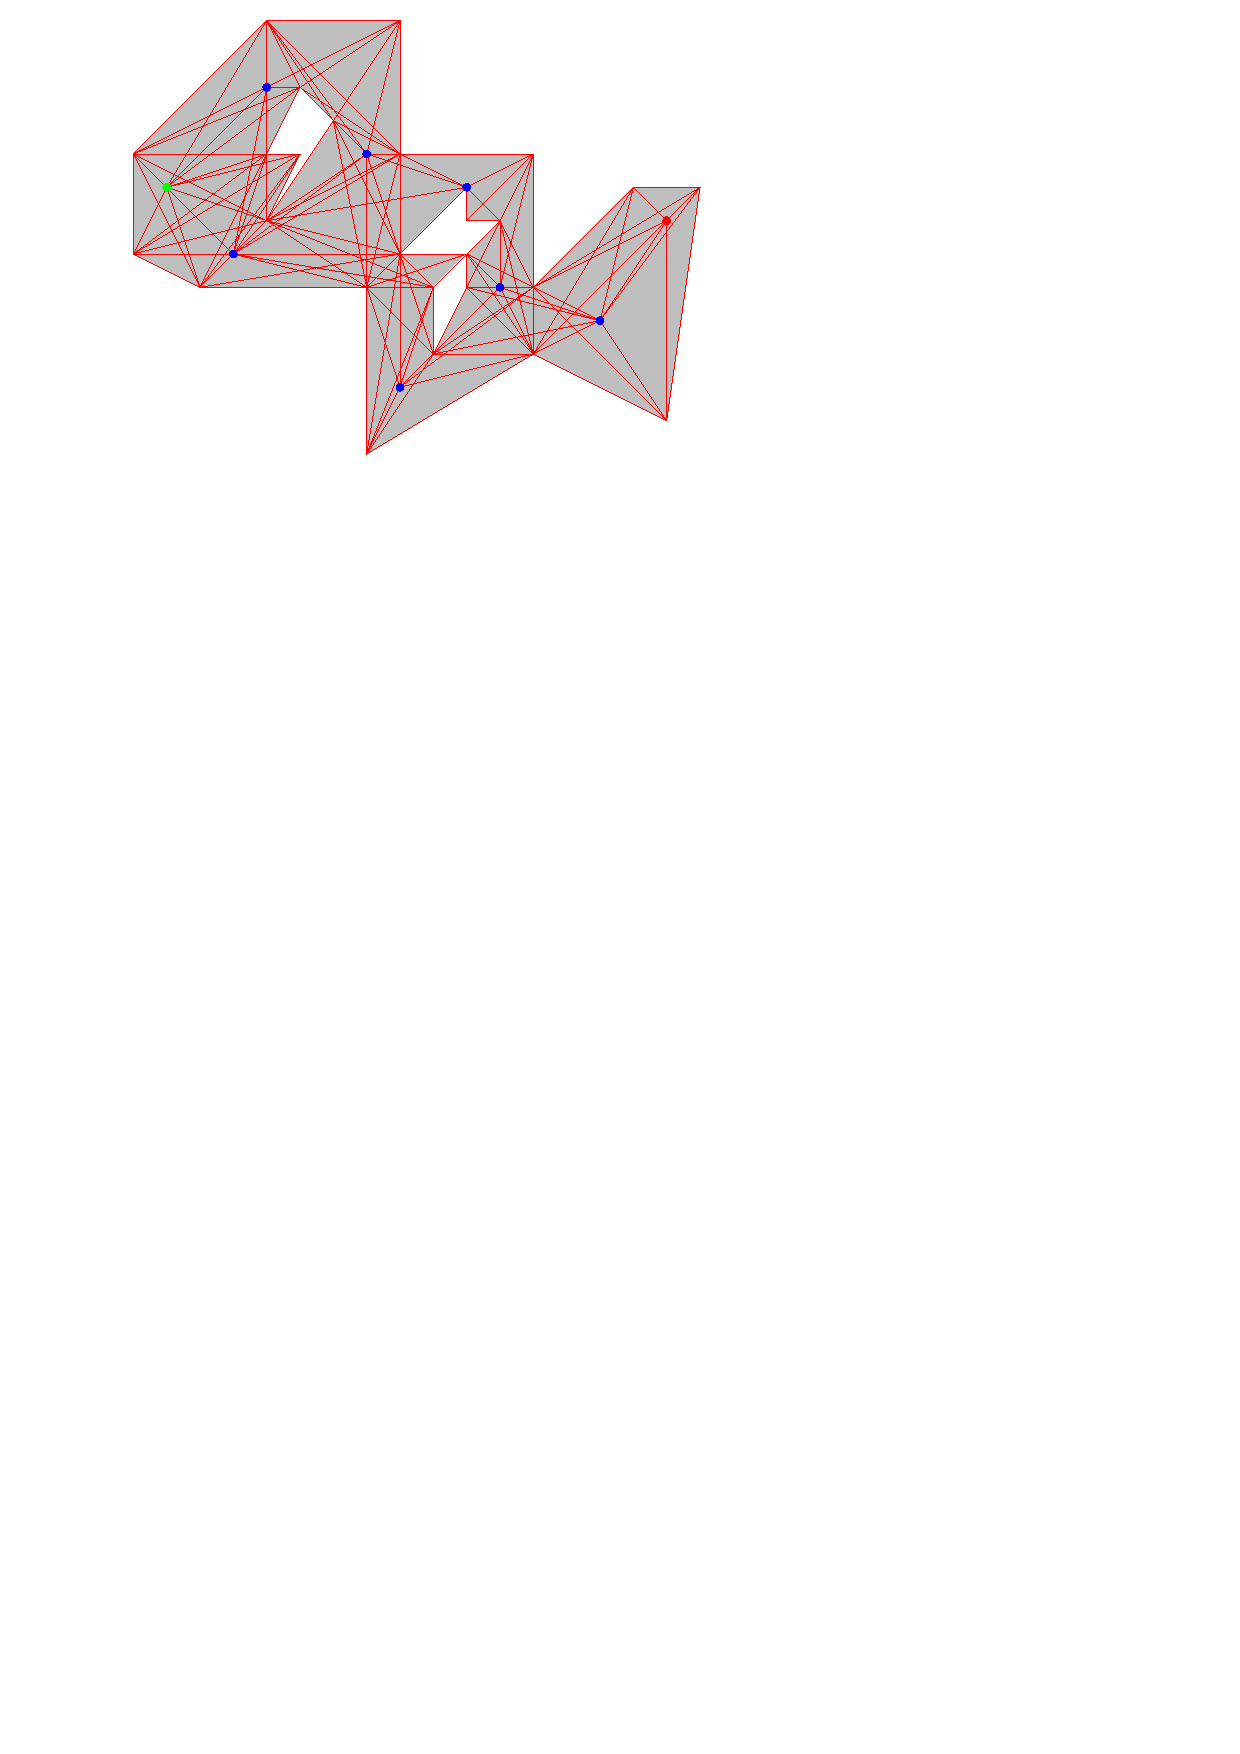
\includegraphics[height=150pt]{graphics/visibility1.pdf}
\end{center}

\end{frame}

\begin{frame}[t]{Computing $G_S$ -- First Attempt}

\vspace{-2em}
\begin{columns}
\begin{column}{0.6\textwidth}
\begin{itemize}
\item For each pair $a, b \in S$, check if $\overline{ab}$ is inside $P$
\item $\Theta(|S|^2)$ segment-in-polygon tests
\item How to check if segment $ab$ is inside $P$?
\end{itemize}
\end{column}
\begin{column}{0.35\textwidth}
\onslide<1>{%
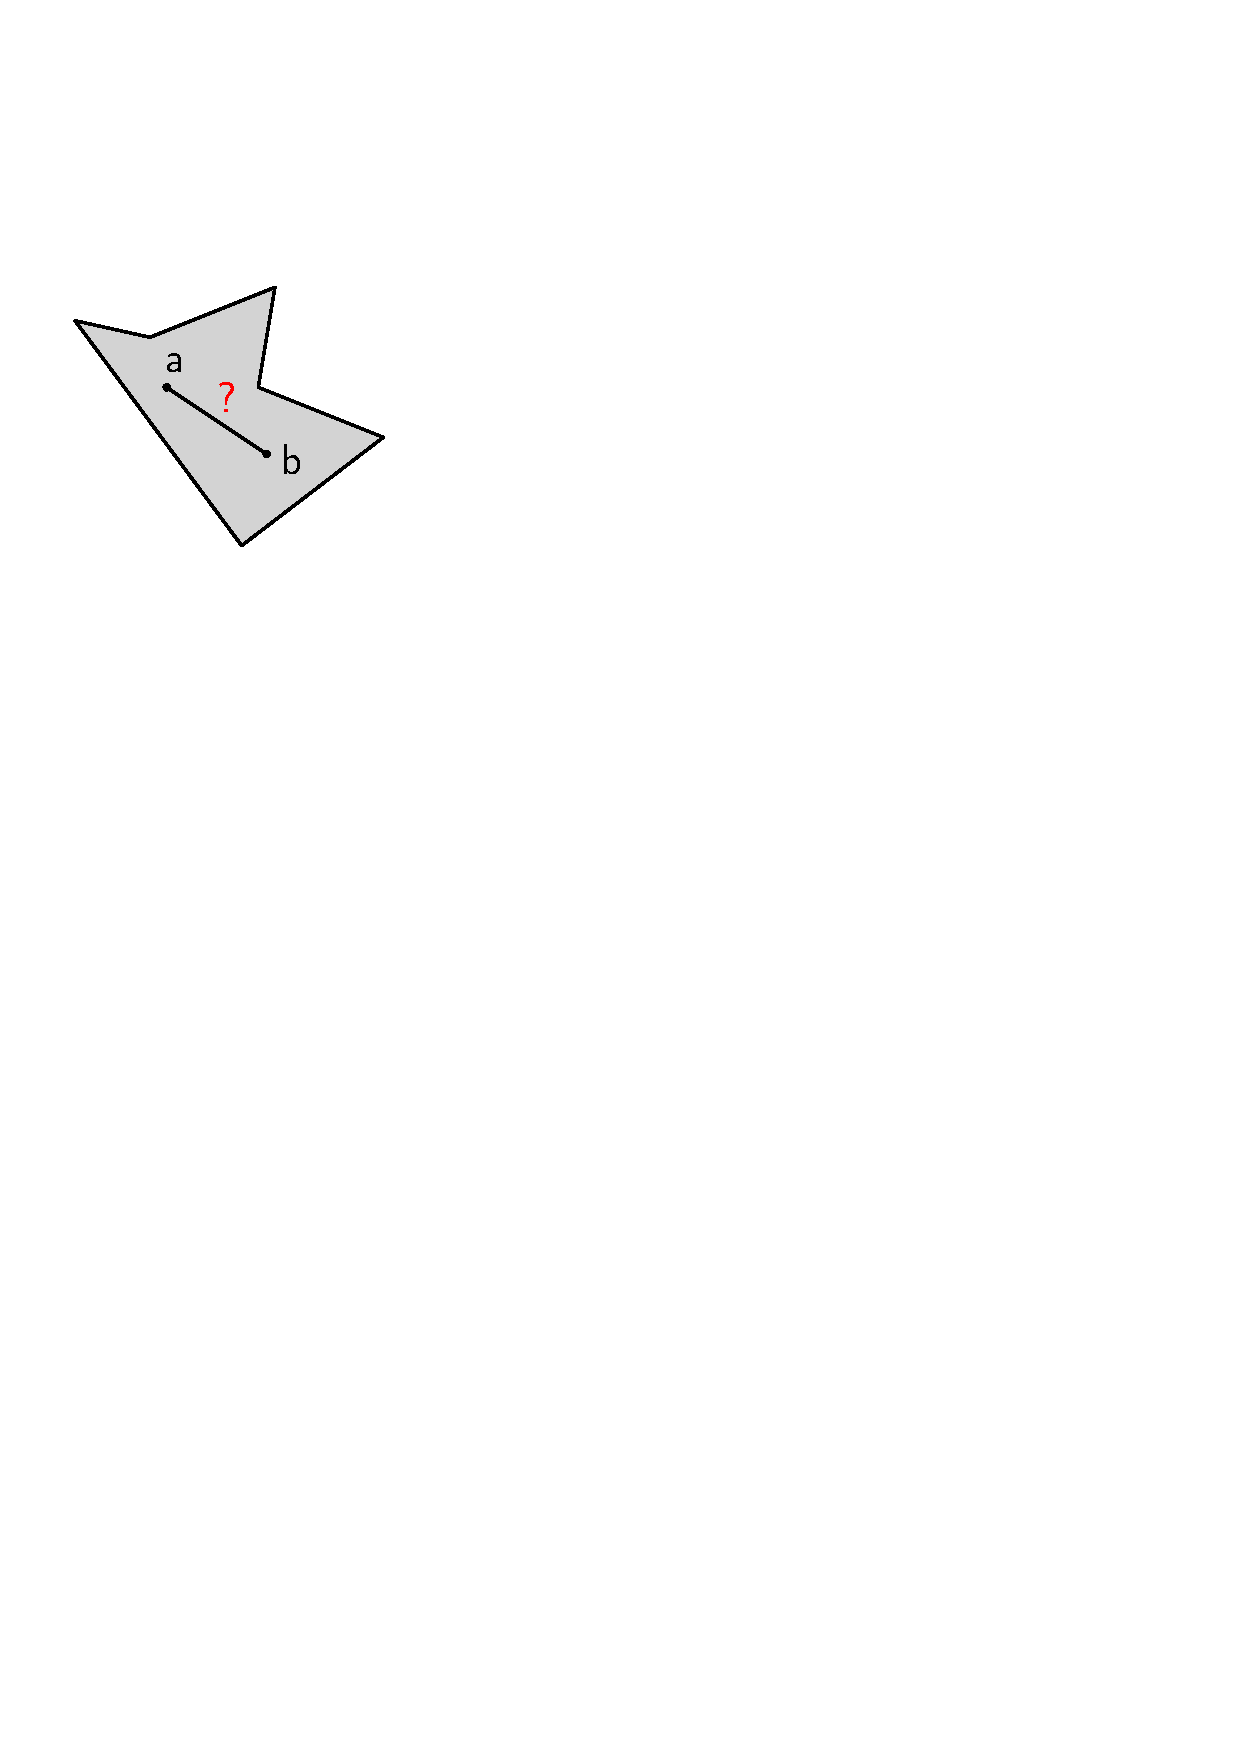
\includegraphics[page=1,height=80pt]{graphics/seg_in_poly2.pdf}%
}%
\end{column}
\end{columns}

\vspace{-1em}
\begin{center}
\begin{columns}
\begin{column}{0.48\textwidth}
\begin{enumerate}
\onslide<2->{%
\item Is there an edge $\overline{pq}$ of $P$ that intersects $\overline{ab}$ in
on the interior? \\
$\rightarrow$ output \textbf{NO}
}

\onslide<3->{%
\item Is the midpoint $(a + b)/2$ outside of $P$? \\
$\rightarrow$ output \textbf{NO}
}

\onslide<4->{%
\item Otherwise, output \textbf{YES}
}
\end{enumerate}
\end{column}

\begin{column}{0.3\textwidth}
\only<2>{%
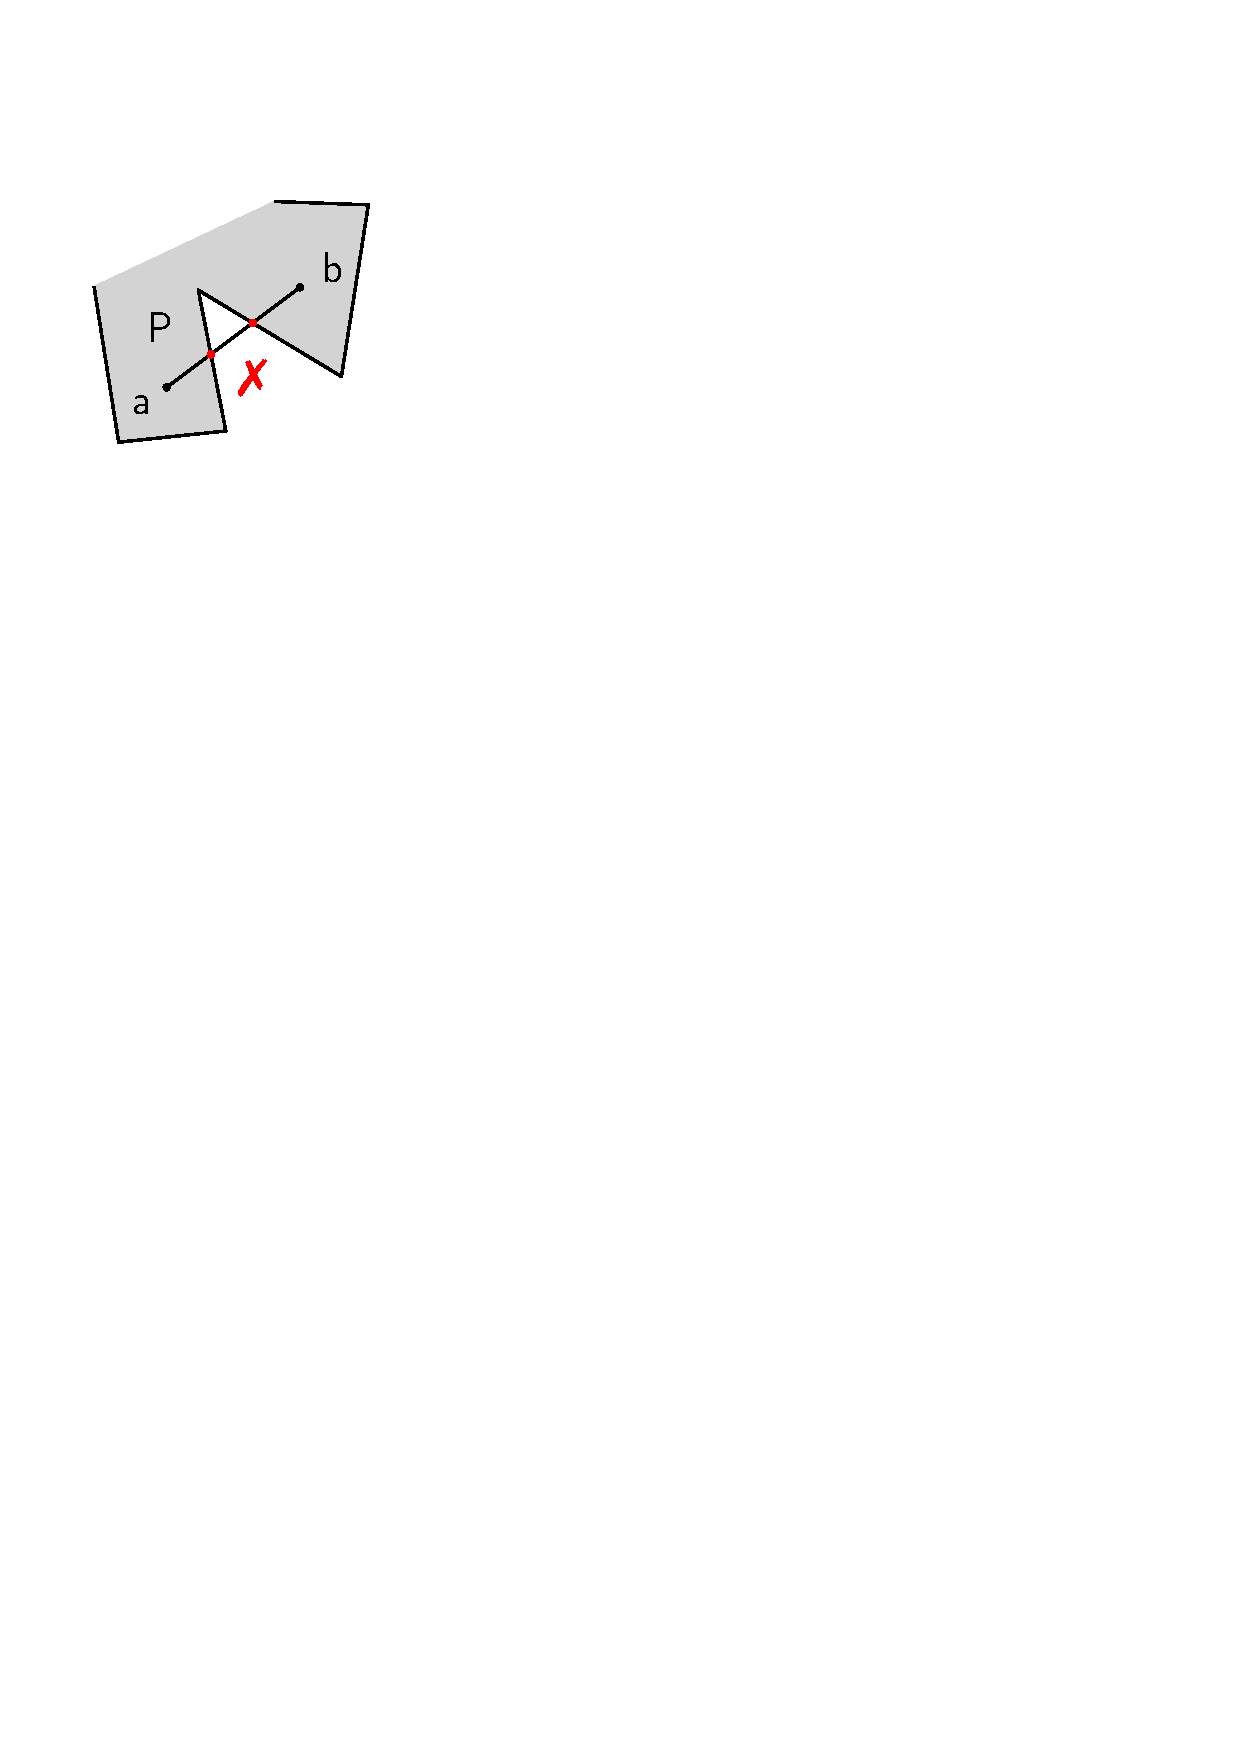
\includegraphics[page=1,height=100pt]{graphics/seg_in_poly.pdf}%
}%
\only<3>{%
\includegraphics[page=2,height=100pt]{graphics/seg_in_poly.pdf}%
}%
\onslide<4->{%
\includegraphics[page=3,height=100pt]{graphics/seg_in_poly.pdf}%
}%
\end{column}
\end{columns}
\end{center}

\onslide<5>{%
Runtime: $\Theta(|S|^2 \cdot |P|)$, dominates runtime of the algorithm
}
\end{frame}

\begin{frame}[t]{Computing $G_S$ -- Second Attempt}
\vspace{-1em}
\begin{itemize}
\item For each $a \in S$, compute points $b$ with $\overline{ab}$ inside $P$ in one pass
\item Use \textbf{Circle-Sweep}: Sort all points/vertices by their angle around $a$
\item Maintain edges of $P$ intersecting the sweep line, sorted by distance
\onslide<17>{
\item Runtime: $\Theta(|S| \cdot n \cdot \log n)$ where $n = |S| + |P|$
\item Now that we have $G_S$, how to solve the problem on a general graph?
}
\end{itemize}
\vspace{-3em}
\begin{center}
\foreach \n in {1,...,15}{%
\only<\n>{%
\includegraphics[page=\n,height=155pt]{graphics/circle_sweep.pdf}%
}%
}
\onslide<16>{%
\includegraphics[page=16,height=155pt]{graphics/circle_sweep.pdf}%
}%
\end{center}

\end{frame}

